\chapter{\textit{Frameworks} MVC e de Persistência}\label{cap:frameworksPersistencia}
\epigraph{``\textit{A persistência é o caminho do êxito}''.}{Charles Chaplin}
\epigraph{``\textit{Não extingua sua inspiração e sua imaginação; não se torne o escravo do seu modelo}''.}{Vincent van Gogh}

\lettrine[lines=4, lhang=0.1, lraise=0, loversize=0.2, findent=0.1em]{\textcolor{corTema}{N}}{ESTE} Capítulo reconstruiremos o ``Sistema de Venda de Produtos'' do Capítulo~\ref{cap:terceiroProjeto} utilizando diversos \textit{frameworks} que tornarão nosso trabalho menos tedioso e mais direto ao ponto!

\vfill

\section{Introdução}

Antes de começarmos a trabalhar, precisamos configurar nosso ambiente de desenvolvimento. Como lidaremos com toda a \textit{stack} de \textit{frameworks} e bibliotecas do Spring, poderíamos utilizar a ferramenta oficial deles para nos auxiliar, a Spring Tool Suite 4. Eu particularmente não sou muito fã, pois ela é baseada na IDE Eclipse que, na minha opinião, é extremamente burocrática e instável, mas como ela é adotada como o padrão da indústria, uma hora ou outra acabamos ter que a adotar. Continuaremos a utilizar o NetBeans como nossa ferramenta padrão, mas você pode testar a Spring Tool Suite caso deseje. No momento em que este texto está sendo escrito existem também versões para o Visual Studio Code (\url{https://code.visualstudio.com/}) a para a IDE Theia (\url{https://theia-ide.org/}). O download de qualquer uma das versões pode ser feito em \url{https://spring.io/tools}.

A primeira coisa que vamos fazer é acessar o site Spring Initializr (\url{https://start.spring.io/}). Nesse site podermos configurar a infraestrutura básica do nosso projeto, que utilizará o Maven (\url{https://maven.apache.org/}) como ferrameta de gerenciamento do projeto. O Maven é suportado atualmente pelas principais IDEs disponíveis. Sendo um projeto Maven, espera-se que todas as IDEs trabalhem de forma semelhante, então teoriacemente podemos trabalhar com mais de uma ferramenta no mesmo projeto. Note que iremos reconstruir o ``Sistema de Venda de Produtos'' do Capítulo\ref{cap:terceiroProjeto}. Vamos começar?

A versão atual da página principal do site do Spring Initializr pode ser vista na Figura~\ref{fig:cap10SpringInitializr}.

\FloatBarrier
\begin{figure}[!htbp]
    \centering
    \caption{Tela principal do site do Spring Initializr}
    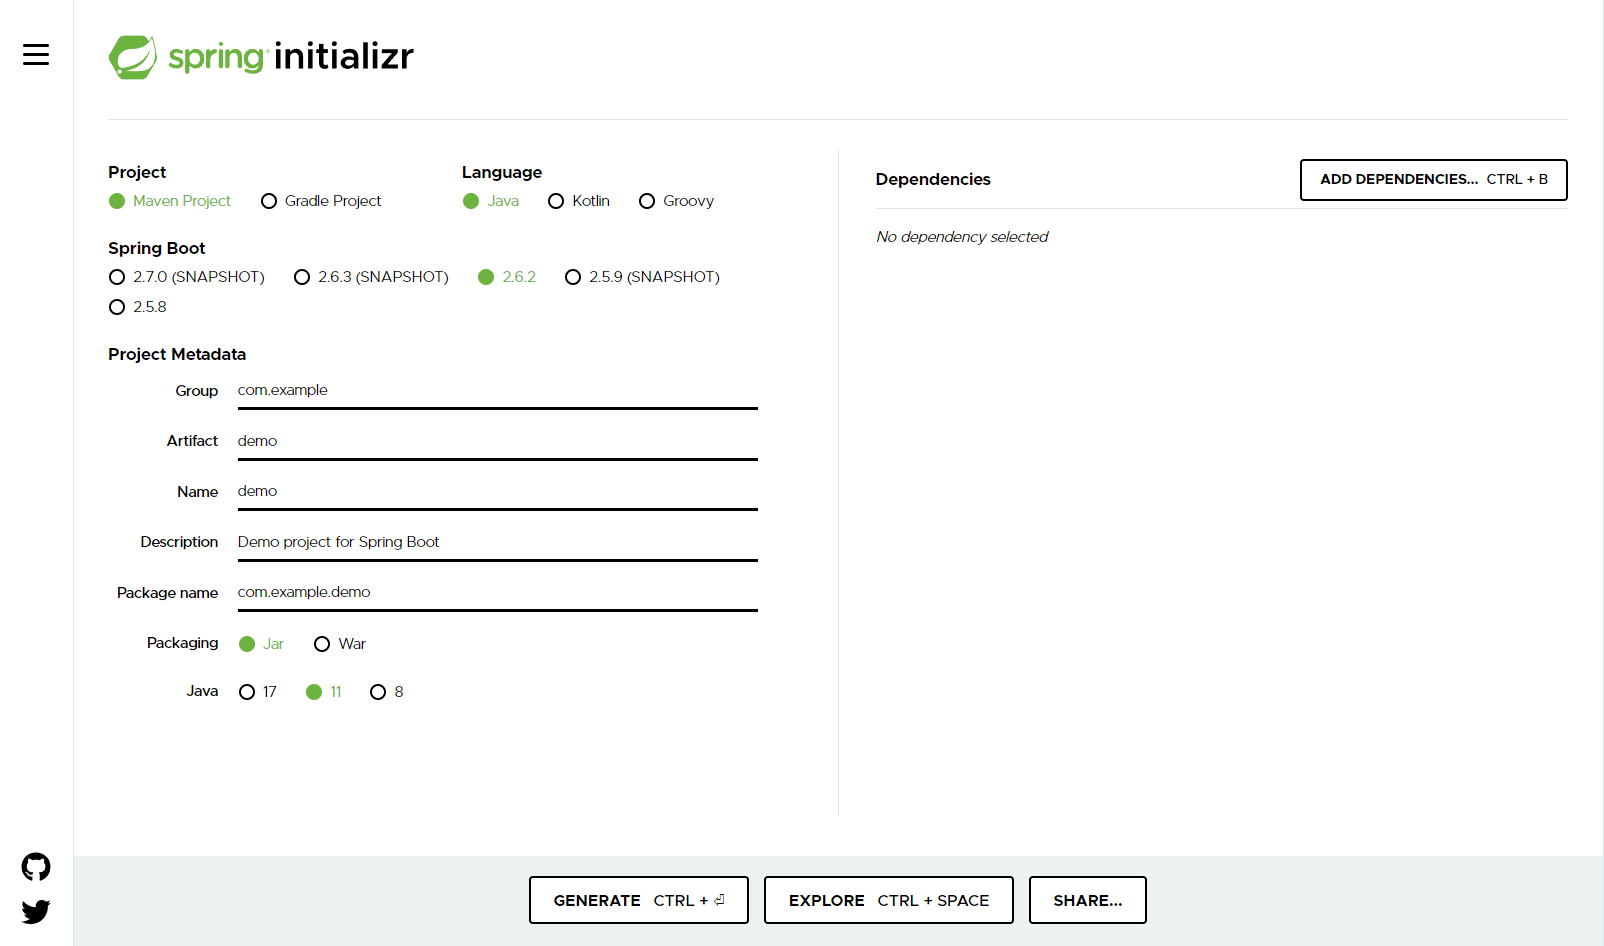
\includegraphics[scale=0.4]{imagens/cap10SpringInitializr}
    \\\textbf{Fonte:} \url{https://start.spring.io/}
    \label{fig:cap10SpringInitializr}
\end{figure}
\FloatBarrier

Basicamente do lado esquerdo temos as opções de configuração do projeto:

\begin{itemize}
    \item \textbf{\textit{Project}:} qual ferramenta de gerencimanto de projetos que será usada (usaremos o Maven);
    \item \textbf{\textit{Language}:} a linguagem de programação utilizada no projeto;
    \item \textbf{\textit{Spring Boot}:} qual a versão do Spring Boot que usaremos;
    \item \textbf{\textit{Project Metadata}:} os metadados do projeto, que envolvem:
    \begin{itemize}
        \item \textbf{\textit{Group}:} nome do identificador do grupo do projeto, normalmente igual ao pacote da organização/empresa do desenvolvedor do projeto, seguindo as regras para noemação de pacotes da linguagem Java (\url{https://docs.oracle.com/javase/specs/jls/se6/html/packages.html#7.7});
        \item \textbf{\textit{Artifact}:} nome do arquivo que será gerado (sem a extensão \texttt{.jar} ou \texttt{.war}) após a construção do projeto e também o identificador que será usado pelo Maven para encontrar a versão compilada e instalada do projeto dentro do repositório local do Maven. Normalmente identificador do artefato tiver mais de uma palavra, separamos as mesmas por hífens;
        \item \textbf{\textit{Name}:} nome do projeto, o que aparecerá na raiz do projeto aberto nas IDEs para identificá-los;
        \item \textbf{\textit{Description}:} breve descrição do objetivo do projeto;
        \item \textbf{\textit{Project name}:} pacote raiz do projeto, usando como prefixo o identificador do grupo. Caso sejam usados hífens~\footnote{O Spring Initializr usará automaticamente o valor do identificador artefato aqui, trazendo hífens, que serão descartados no pacote final}, eles serão suprimidos no projeto gerado;
        \item \textbf{\textit{Packaging}:} tipo de empacotamento que será feito. Arquivos \texttt{.jar} podem ser executados localmente e arquivos \texttt{.war} são destinados à implantação em servidores de aplicações e/ou containeres de Servetls;
        \item \textbf{\textit{Java}:} a versão do Java que se quer usar. Note que apenas as versões \textit{Long-Term Support} (LTS) aparecem e, além disso, você precisa ficar atento para ter um JDK de versão igual ou superior instalado na máquina de desenvolvimento.
    \end{itemize}
\end{itemize}

Sabendo disso, vamos agora preparar o nosso projeto de acordo com o apresentado na Figura~\ref{fig:cap10SpringInitializrConfProjeto01}:

\FloatBarrier
\begin{figure}[!htbp]
    \centering
    \caption{Definição das propriedades do projeto}
    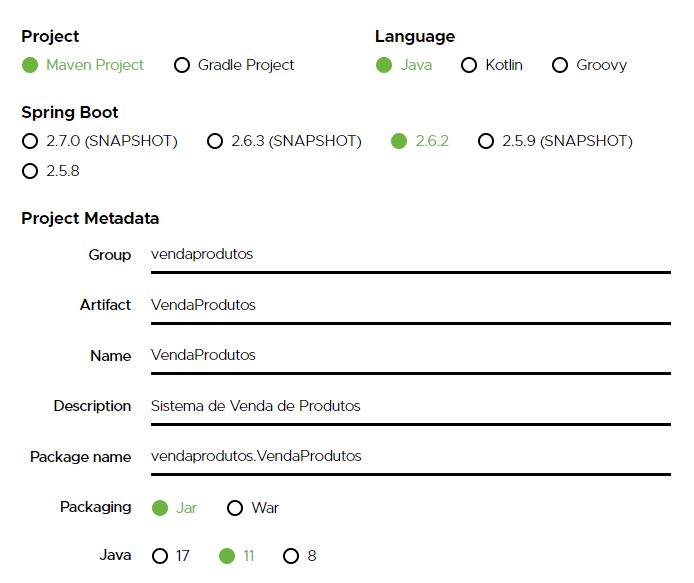
\includegraphics[scale=0.7]{imagens/cap10SpringInitializrConfProjeto01}
    \\\textbf{Fonte:} \url{https://start.spring.io/}
    \label{fig:cap10SpringInitializrConfProjeto01}
\end{figure}
\FloatBarrier

Ou seja:

\begin{itemize}
    \item \textbf{\textit{Project}:} usaremos o Maven;
    \item \textbf{\textit{Language}:} programaremos em Java;
    \item \textbf{\textit{Spring Boot}:} a última versão estável do Spring Boot, nesse caso, a 2.6.2. Note que isso pode variar de acordo com a época que você estiver lendo esse texto;
    \item \textbf{\textit{Project Metadata}:} os metadados do projeto, que envolvem:
    \begin{itemize}
        \item \textbf{\textit{Group}:} usaremos \texttt{dsoc7}, que é a sigla da disciplina para a qual esse livro foi desenvolvido incialmente, mas em um caso real, você deve preencher com a notação de domínio inverso da empresa ou instituição para a qual estiver desenvolvendo o projeto. Por exemplo, se a instuição tem o domínio \texttt{ifsp.edu.br}, você deverá preencher o identificador do grupo com \texttt{br.edu.ifsp}. Caso seja um projeto pessoal e você possuir um domínio, a regra é a mesma. Eu por exemplo tenho o domínio \texttt{davidbuzatto.com.br}, então meu identificador de grupo, para um projeto pessoal, deve ser \texttt{br.com.davidbuzatto};
        \item \textbf{\textit{Artifact}:} usaremos \texttt{venda-produtos-spring};
        \item \textbf{\textit{Name}:} o nome preencheremos com \texttt{VendaProdutosSpring}, que é o que aparecerá no NetBeans na raiz do projeto. Aqui em um caso real você poderia usar espaços para nomear o projeto. Eu prefiro sem espaços;
        \item \textbf{\textit{Description}:} preencher com Sistema de Venda de Produtos Usando Spring Boot;
        \item \textbf{\textit{Project name}:} aqui o Spring Initializr já deve ter preenchido com a concatenção do identificador do grupo e do identificador do artefato, ficando \texttt{dsoc7.venda-produtos-spring}. Na criação do projeto esses hífens serão retirados, pois nomes de pacotes em Java não podem ter hífem;
        \item \textbf{\textit{Packaging}:} usaremos empacotamento em \texttt{.jar};
        \item \textbf{\textit{Java}:} usaremos o Java 11.
    \end{itemize}
\end{itemize}

Com isso feito temos a configuração básica do projeto pronta, mas ainda precisamos adicionar as primeiras dependências que utilizaremos. As dependências são basicamente as biblitecas que usaremos no projeto. A vantagem de usar um sistema de gerenciamento de projetos como o Maven é que, ao adicionarmos dependências no projeto, ele se encarregará de carregar todas as dependências que uma dependência depende, inclusive com as versões apropriadas! Nossa vida fica muito mais fácil sem precisar ficar lidando com definição de bibliotecas e isso é um super avanço na produtividade!

Para adicionar uma dependência, clique no botão \destaque{\textit{ADD DEPENDENCIES...}}. Ao fazer isso, um diálogo aparecerá, onde você poderá escolher as dependências do projeto. Ao encontrar a dependência desejada, basta clicar nela que ela será inserida na lista de dependências do projeto. Você pode procurar pelas dependências rolando a lista ou então pesquisando na caixa de texto acima. No nosso projeto utilizaremos sete dependências, apresentadas na Figura~\ref{fig:cap10SpringInitializrConfProjeto02} e descritas a seguir.

\FloatBarrier
\begin{figure}[!htbp]
    \centering
    \caption{Definição das dependências do projeto}
    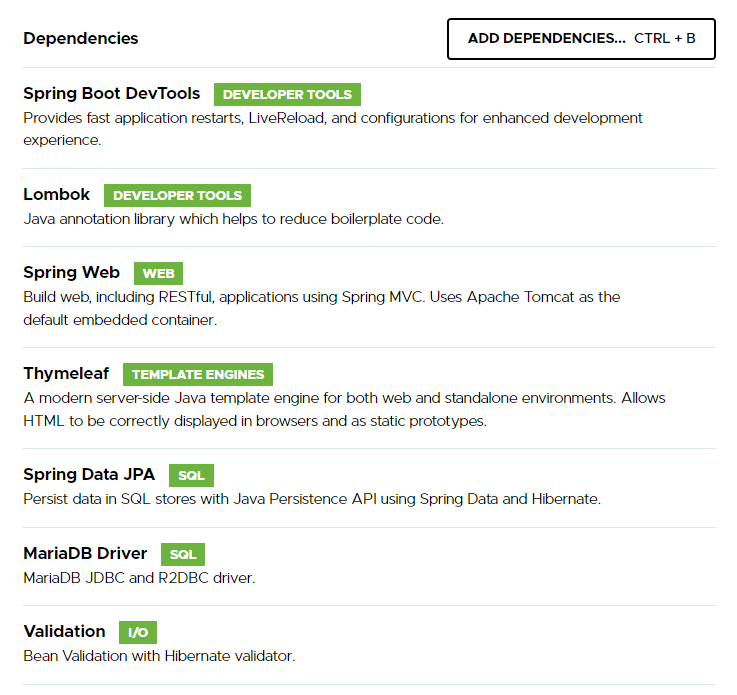
\includegraphics[scale=0.7]{imagens/cap10SpringInitializrConfProjeto02}
    \\\textbf{Fonte:} \url{https://start.spring.io/}
    \label{fig:cap10SpringInitializrConfProjeto02}
\end{figure}
\FloatBarrier

\begin{itemize}
    \item \textbf{Spring Boot DevTools:} auxília no desenvolvimento de aplicações usando Spring Boot, permitindo reinicialização rápida, integração com LiveReload etc;
    \item \textbf{Lombok:} é uma biblioteca de anotações que nos ajuda na criação automática de código padronizado como getters, setters, construtores etc;
    \item \textbf{Spring Web:} construção de aplicações Web usando o padrão de projeto MVC através do \textit{framework} Spring MVC, além da criação de Web Services RESTful;
    \item \textbf{Thymeleaf:} é uma \textit{template engine} que permite a definição de modelos para a criação de interfaces gráficas usando HTML, diminuindo a duplicidade de código e facilitando a manutenção.
    \item \textbf{Spring Data JPA:} \textit{framework} para persistência de dados usando Hibernate e a Java Persistence API (JPA);
    \item \textbf{MariaDB Driver:} driver de conexão com MariaDB, o SGBD que estamos utilizando neste livro;
    \item \textbf{Validation:} permite a validação de objetos de dados que serão gerenciados pela aplicação (já fizemos algo parecido, você se lembram?);
\end{itemize}

Agora com o inicializador do projeto configurado, clique no botão \destaque{GENERATE}. Ao fazer isso, um arquivo \texttt{.zip} será baixado, com o nome de \texttt{venda-produtos-spring.zip}. No local onde foi salvo, descompacte-o. Abra o NetBeanse realize o procedimento de abrir projetos. Vá à pasta onde o arquivo foi descompactado. Você notará que o NetBeans reconhecerá um projeto Maven ali. Selecione-o e abra-o.

As configurações iniciais do projeto gerado no Spring Initilizr podem ser compartilhadas. Sendo assim, se você quiser, pode usar o \textit{link} abaixo para fazer o \textit{download} do projeto com as mesmas configurações apresentadas.

\url{https://start.spring.io/#!type=maven-project&language=java&platformVersion=2.6.2&packaging=jar&jvmVersion=11&groupId=dsoc7&artifactId=venda-produtos-spring&name=VendaProdutosSpring&description=Sistema%20de%20Venda%20de%20Produtos%20Usando%20Spring%20Boot&packageName=dsoc7.venda-produtos-spring&dependencies=devtools,lombok,web,thymeleaf,data-jpa,mariadb,validation}

Provavelmente, após abrir o projeto, seu NetBeans vai demorar alguns minutos --pode demorar bastante na verdade-- para baixar o índice central do Maven e prepará-lo no seu computador. Após esse processo, seu NetBeans vai ``reclamar'', informando que o repositório do Maven local não tem uma cópia das dependências do projeto. Veja na Figura~\ref{fig:cap10ConfProjeto03} o que provavelmente aparecerá, ou seja, um sinal de aviso (\textit{warning}) no ícone do projeto.

\FloatBarrier
\begin{figure}[!htbp]
    \centering
    \caption{Resolução de problema do projeto criado}
    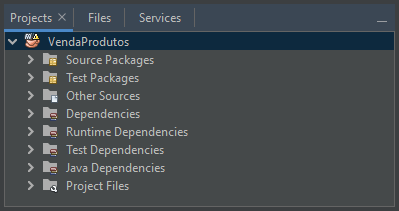
\includegraphics[scale=1]{imagens/cap10ConfProjeto03}
    \\\textbf{Fonte:} Elaborada pelo autor
    \label{fig:cap10ConfProjeto03}
\end{figure}
\FloatBarrier

Para resolvermos isso, faremos algo que talvez você já tenha feito para outras situações. Clique com o botão direito no projeto e escola a opção \destaque{\textit{Resolve Project Problems...}} do menu de contexto. Fazendo isso, um diálogo aparecerá com um ou mais itens com o texto ``\textit{Some dependency artifacts are not in the local repository}'', indicando o problema encontrado. Clique no botão \destaque{\textit{``Resolve''}}. O Maven vai começar a realizar o processo de ``Priming'' (preparação) do projeto, prepararando e baixando todas as dependências. Essa preparação pode demorar um pouco também. Você saberá que o processo terminou quando aparecer ``BUILD SUCESS'' na saída do NetBeans e quando o diálogo da solução dos problemas do projeto apresentar o problema apontado anteriormente com um ``check'' ou ``tick'' verde. Clique em Close.

explicar estrutura do projeto

falar  other sources para mostrar como diretórios

rodar pela primeira vez

criar um index

configurar o WebConfig

como executar

como associar ao navegador com LiveReload

arquivo de configurações do Spring Boot

falar do POM


\section{Hibernate, JPA, Validações e Lombok}

criação das entidades
carga inicial no banco


\section{Spring MVC}

criação dos controladores e páginas com thymeleaf


\subsection{Outros \textit{Frameworks} MVC}

%Falar brevemente de: JavaServer Faces (JSF), Struts, VRaptor etc.


\section{\textit{Web Services RESTful}}

criação de controladores rest e consumir API usando Javascript.

talvez uma inserção e uma listagem?


\section{Resumo}

\section{Exercícios}

\section{Projetos}
